\chapter{Background}
\label{cha:background}

%\section{Information Security}
%\label{sec:information_security}

%Nowadays, information is one of the most important assets in enterprises. All employees create and work with information day by day. This information can be essential for the success of enterprises. According to that, insufficiently protected information can be a high-risk factor and even be existence-threatening for enterprises. \cite{bsi} Besides important enterprise assets, personal data additionally has to be considered in information security, particularly regulated by the General Data Protection Regulation (\textbf{GDPR}). \cite{EU-DSGVO} information security is a dynamically evolving field according to technological development. It defines multiple information security goals, that can determine to what extent IT-Systems have reached information security. The most important information security goals are \emph{confidentiality}, \emph{authenticity}, \emph{availability}, and \emph{integrity}. \cite{schutzziele_bedner}

%\subsection{Confidentiality}
%\label{subsec:confidentiality}

%Confidentiality in IT-Systems means, that information is only available to authorized individuals. This is mostly a defined group of individuals. Compliance with confidentiality requires an access control mechanism, to distinguish authorized and unauthorized individuals, depending on their access rights. Another important instrument for confidentiality is the encryption of information. The goal is to obfuscate information in an unreadable way so that only authorized individuals with a corresponding key can decrypt and interpret the information. \cite{schutzziele_bedner}

%\subsection{Authenticity}
%\label{subsec:authenticity}

%Authenticity in IT-Systems is responsible for the identification of a user by control mechanism and the verification, that data and information derives from a valid source. The identification is mostly based upon a set of credentials that is owned by and explicitly identifies him. For example, this could be a user password, biometric fingerprints, or identification cards such as a personal identity card. In IT-Systems, identification is mostly done during a login, by verifying the credentials of a user. Furthermore, it is important that the identity is not only guaranteed at the beginning of a communication but also during the entire communication. \cite{schutzziele_bedner}

%\subsection{Availability}
%\label{subsec:availability}

%Availability directly concerns applications and services as well as data and assets that are managed inside applications. It ensures that applications and services are in operation at any time and that users can access data and assets at any time while guaranteeing their completeness and correctness. The maximum desirable availability is of course 100\%. This is calculated by the relation between the actual running time and the expected running time. The time, when the application is not running and not available is defined as downtime. Availability is often part of a Service-Level-Agreement (\textbf{SLA}), that defines the application's availability by a contract between the service provider and the customer. \cite{schutzziele_bedner}

%\subsection{Integrity}
%\label{subsec:integrity}

%Integrity ensures that data and assets are complete and available. Secondly, it ensures that data and assets are correct and tamper-free and that applications and services are working as intended. Integrity is reached when data and assets are tamper-free during processing and transmission and unauthorized parties are not able to manipulate them. Manipulations include replacing, inserting, or deleting data. There are a variety of tools and methods to ensure tamper-free data. For example, cryptographic hash methods are used to sign data and subsequently recognize manipulated data when verifying the signature. \cite{schutzziele_bedner}

\section{Marketplace}
\label{sec:marketplace}

% marketplace & trading platform interchangeable
% real world examples

%agora
%Data privacy: no party can learn any information about the
%raw data of the generators, apart from the function output
%that is learnt by the broker and paying consumers.
%Output verifiability: no broker can successfully sell an incorrect
%or falsified result to a consumer.
%Atomicity of payments: no entity can avoid paying for services,
%i.e., generators are reimbursed for their data and
%brokers are paid for providing function outputs.

% drynx
% A. Use Cases We illustrate Drynx’s utility in the medical sector, as it is a paradigmatic example where privacy is paramount and data sharing is needed. Recently, multiple initiatives have emerged to realize the promise of personalized medicine and to address the challenges posed by the increasing digitalization of medical data [48], [49], [50]. In this context, the ability to share highly sensitive medical data while protecting patients’ privacy is becoming of primary importance. We illustrate the possible use of Drynx in two specific settings that cover most medical data sharing scenarios: (1) Hospital Data Sharing (HDS), where multiple hospitals enable statistical computations and the training of machine-learning models across their datasets of patients (e.g., [50], [51]), and (2) Personal Data Sharing (P DS), where a medical institute runs studies, e.g., on heart issues, by directly computing on data collected from people’s wearables (e.g., [52], [53]).


% review system hinzufügen (Towards a Decentralized Data Marketplace for Smart Cities hat auch ratings, gucken welche noch ratings haben)
% ramachandranDecentralizedDataMarketplace2018 - rating system to ensure trust
% idmob auch ratings: a voting system to rank data sources


\begin{figure}[!htb]
    \centering
    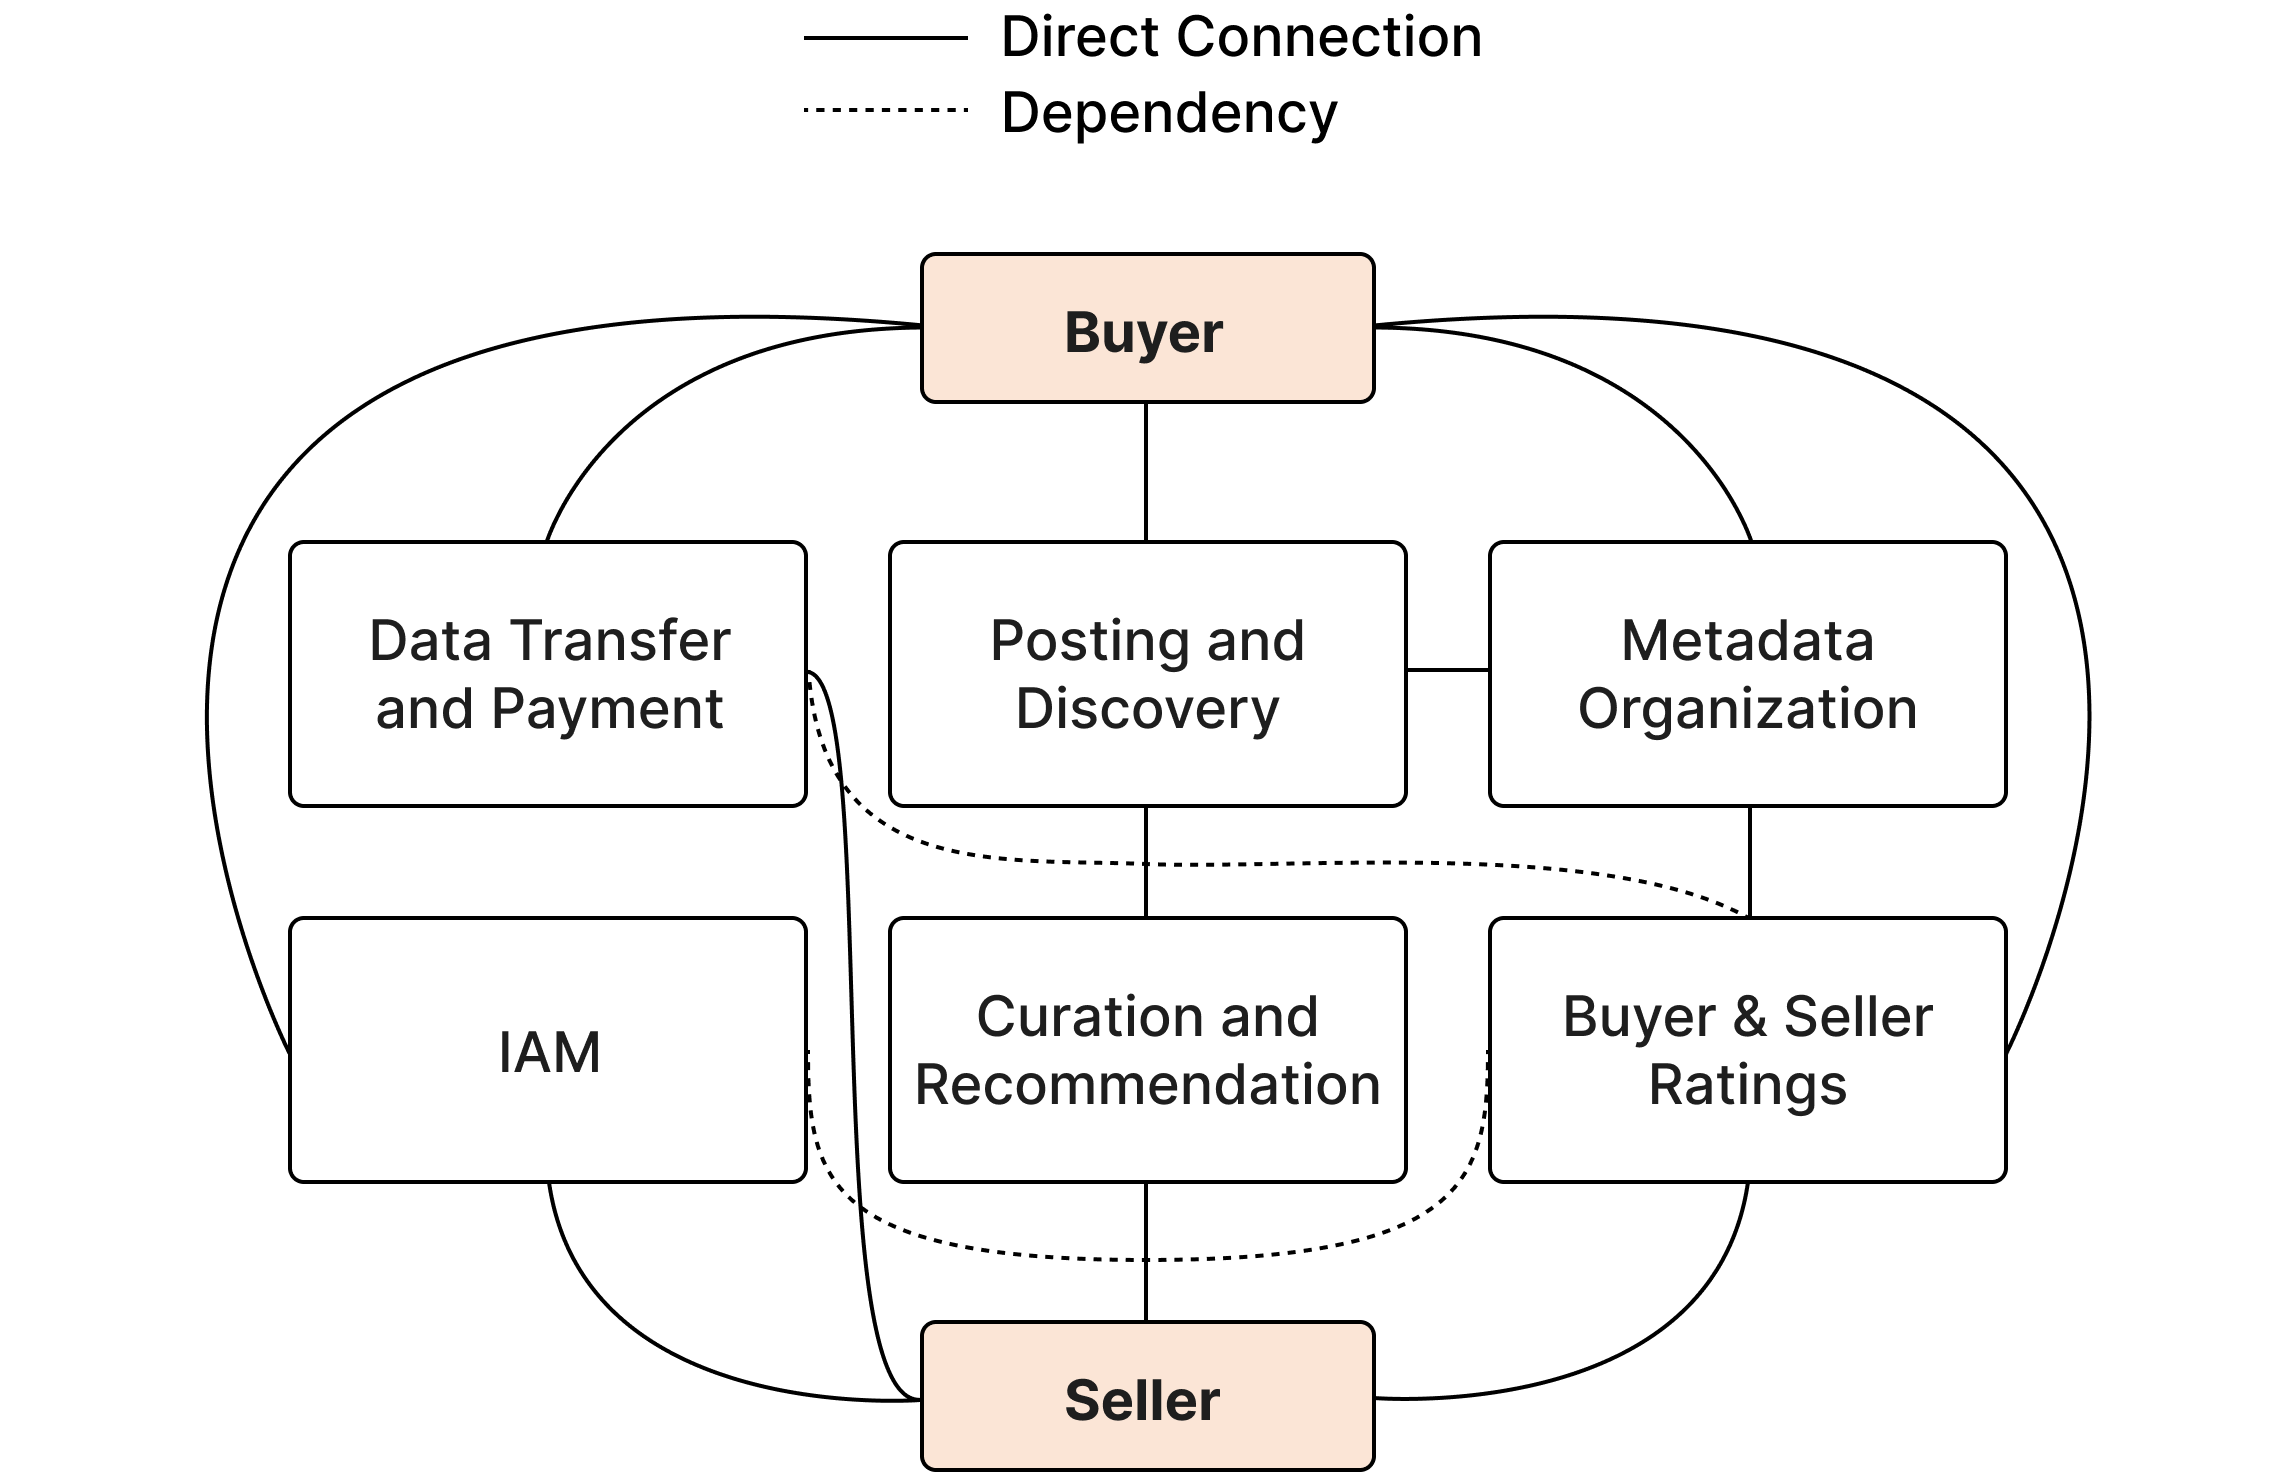
\includegraphics[width=13cm]{images/components-clean.png}
    \caption[Key components and features of a digital data trading platform]{Key components and features of a digital data trading platform. All components in red show the aspired enhancements by the contributions of this thesis.}
    \label{fig:components}
\end{figure}

\section{Blockchain}
\label{sec:blockchain}

Lorem ipsum dolor sit amet, consetetur sadipscing elitr, sed diam nonumy eirmod tempor invidunt ut labore et dolore magna aliquyam erat, sed diam voluptua. At vero eos et accusam et justo duo dolores et ea rebum. Stet clita kasd gubergren, no sea takimata sanctus est Lorem ipsum dolor sit amet. Lorem ipsum dolor sit amet, consetetur sadipscing elitr, sed diam nonumy eirmod tempor invidunt ut labore et dolore magna aliquyam erat, sed diam voluptua. At vero eos et accusam et justo duo dolores et ea rebum. Stet clita kasd gubergren, no sea takimata sanctus est Lorem ipsum dolor sit amet.

Lorem ipsum dolor sit amet, consetetur sadipscing elitr, sed diam nonumy eirmod tempor invidunt ut labore et dolore magna aliquyam erat, sed diam voluptua. At vero eos et accusam et justo duo dolores et ea rebum. Stet clita kasd gubergren, no sea takimata sanctus est Lorem ipsum dolor sit amet. Lorem ipsum dolor sit amet, consetetur sadipscing elitr, sed diam nonumy eirmod tempor invidunt ut labore et dolore magna aliquyam erat, sed diam voluptua. At vero eos et accusam et justo duo dolores et ea rebum. Stet clita kasd gubergren, no sea takimata sanctus est Lorem ipsum dolor sit amet.

Lorem ipsum dolor sit amet, consetetur sadipscing elitr, sed diam nonumy eirmod tempor invidunt ut labore et dolore magna aliquyam erat, sed diam voluptua. At vero eos et accusam et justo duo dolores et ea rebum. Stet clita kasd gubergren, no sea takimata sanctus est Lorem ipsum dolor sit amet. Lorem ipsum dolor sit amet, consetetur sadipscing elitr, sed diam nonumy eirmod tempor invidunt ut labore et dolore magna aliquyam erat, sed diam voluptua. At vero eos et accusam et justo duo dolores et ea rebum. Stet clita kasd gubergren, no sea takimata sanctus est Lorem ipsum dolor sit amet.

Lorem ipsum dolor sit amet, consetetur sadipscing elitr, sed diam nonumy eirmod tempor invidunt ut labore et dolore magna aliquyam erat, sed diam voluptua. At vero eos et accusam et justo duo dolores et ea rebum. Stet clita kasd gubergren, no sea takimata sanctus est Lorem ipsum dolor sit amet. Lorem ipsum dolor sit amet, consetetur sadipscing elitr, sed diam nonumy eirmod tempor invidunt ut labore et dolore magna aliquyam erat, sed diam voluptua.

\subsection{Smart Contracts}
\label{subsec:sc}

Smart Contracts were first mentioned in 1994 by Nick Szabo, as a "computerized transaction protocol that executes the terms of a contract" \cite{Szabo_1997}. When contract terms are met, computer code executes exactly as designed in a \emph{trustless} and \emph{self-enforcing}-manner, without the need for a central authority or any other \acrshort{ttp}. It can be compared to a vending machine, which automatically drops a selected product, assuming pre-determined conditions are met, i.e. the product is in stock and the price is covered \cite{Szabo_1997}. This creates a predictable outcome.

In 2014, Vitalik Buterin \cite{buterinNEXTGENERATIONSMART} brought the idea of smart contracts to the Ethereum blockchain. Next to payments, it was possible to deploy and execute computer programs on Ethereum, in a tamper-proof and distributed manner without trusting a central server. Every smart contract has its own address on the blockchain, which can be targeted by an \acrfull{eoa} or another smart contract in the form of a transaction. A transaction can trigger smart contract functions, which can be (i.) read-only; (ii.) state-changing in the smart contract's memory; (iii.) call a function of another smart contract; or (iv.) deploy a new smart contract. The runtime is called the \acrfull{evm} which implements a turing-complete programming language in which smart contracts are written. To prevent inconsistent state on the blockchain, smart contracts need to satisfy \emph{determinism} and \emph{termination}.

\begin{enumerate}
    \item \emph{Determinism}: Each node in the network produces the same result given the same input to guarantee consensus. Hence, access to the filesystem and network is forbidden.
    \item \emph{Termination}: To prevent a \acrfull{dos} by infinite loops or long-running transactions, Ethereum adds the concept of gas to force transactions to terminate. This is a circumvention of the halting problem for turing-complete programming languages. If the maximum amount of gas allocated for a transaction runs out before the transaction is finished, the execution terminates and the state reverts to the previous state before the transaction. This is known as the transaction gas limit. Besides that, the block gas limit specifies the maximum amount of gas for \emph{all} transactions.
\end{enumerate}

\subsection{Tokenization}
\label{subsec:tokenization}

Next to the native currency of a blockchain such as Ether for Ethereum, other tokenized assets exist on top of the underlying blockchain. Tokenization is the process of transforming something valuable, i.e. a scarce digital or physical asset that is ownable, into a digital token, governed by a smart contract \cite{chenBlockchainTokensPotential2018}. Creating a new token is called \emph{minting} and destroying it is called \emph{burning}. In contrast to fiat money, tokens generally have a fixed supply to prevent inflation \cite{chenBlockchainTokensPotential2018}. Furthermore, a token can be (i.) \emph{tangible} if it is something physical or touchable such as gold, a car, or an artwork; (ii.) \emph{intangible} if it is something digital or untouchable such as a cryptocurrency or voting right; (iii.) \emph{fungible} if it is something interchangeable, divisible and not
unique such as fiat money, Bitcoin, or gold; and (iv.) \emph{non-fungible} if it is unique, not interchangeable, and not divisible such as an artwork or a house. The morphological token classification framework \cite{freniTokenomicsBlockchainTokens2022} provides a more fine-grained analysis among multiple domains and dimensions.

Coarsely, tokens can be classified as currency -, utility -, and security tokens, among others:

\begin{enumerate}
    \item \emph{Currency Token}: A currency token is used for payments and thus tradeable and spendable. Next to the most prominent example Bitcoin, there are for example other stable coins such as Thether\footnote{https://tether.to/en/} and USD Coin\footnote{https://www.centre.io/usdc}, being a substitute of the US dollar. 
    \item \emph{Utility Token}: A utility token has a specific purpose, for example giving preferred access to a service or qualify the owner for bonuses and prices. The value of the token is not tied to the companie's success, but it arouses interest to the companie's products and services.
    \item \emph{Security Token}: A security token is typically a share or voting right in a company as an investment. Hence, the value may vary according to the underlying asset. Just like traditional securities, the owner gets specific rights with regards to the company.
\end{enumerate}

Tokenization can have multiple benefits. For example, fractionalization of an underlying asset in a token can positively influence the range of investment opportunities and liquidity. In this way, it is possible to invest in 1/20 of an expensive art piece for example. Furthermore, tokenization can reduce costs and transaction times due to less intermediaries, less bureaucracy, and automated workflows with smart contracts. Lastly, blockchain inherently is transparent and immutable and thus increases trust since users can reliably trace the origin of an asset, its history and changes in ownership. 

\subsubsection{ERC-20}
\label{subsubsec:erc20}

An \acrfull{erc20} token is a technical standard for a fungible token as a smart contract on the Ethereum blockchain. Therefore, \acrshort{erc20} tokens are interchangeable, not unique, and transferable. They can represent anything, but mostly some kind of asset, access right, reputation point, voting right, or even a new cryptocurrency. The \acrshort{erc20} standard was proposed in 2015 and implemented as an \acrfull{eip20}\footnote{https://eips.ethereum.org/EIPS/eip-20} in 2017. The core implementation of an \acrshort{erc20} compliant token consists of 6 functions and 2 events, as depicted below in Listing \ref{lst:erc20-implementation}.\vspace{3mm}

\begin{lstlisting}[language=Solidity,caption={Core interface of an ERC-20 compliant token},label={lst:erc20-implementation}]
// amount of tokens in circulation
function totalSupply() public view returns (uint256)
// amount of tokens owned by an account
function balanceOf(address _owner) public view returns (uint256 balance)
// transfers amount of tokens from the owner to a recipients address
function transfer(address _to, uint256 _value) public returns (bool success)
// transfers amount of tokens from one address to another on behalf of owner
function transferFrom(address _from, address _to, uint256 _value) public returns (bool success)
// approves an address to spend a specific amount of tokens from owner
function approve(address _spender, uint256 _value) public returns (bool success)
// returns remaining amount of tokens allowed to spend from owner
function allowance(address _owner, address _spender) public view returns (uint256 remaining)
// emitted on a successful transfer of tokens
event Transfer(address indexed _from, address indexed _to, uint256 _value)
// emitted when a spender is approved to spend tokens on behalf of owner
event Approval(address indexed _owner, address indexed _spender, uint256 _value)
\end{lstlisting}

\subsubsection{ERC-721}
\label{subsubsec:erc721}

\acrshort{erc721}\footnote{https://eips.ethereum.org/EIPS/eip-721} compliant tokens are more complex than \acrshort{erc20} tokens, because they are unique and not interchangeable. Hence, each \acrshort{erc721} token can have a different value than another token. For example, a seat in the front row of a concert might have a different value than a seat in the back row. This property of distinctness makes it a so called \acrfull{nft}. According to that, the core implementation of an \acrshort{erc721} compliant token consists of 8 functions and 3 events, as depicted below in Listing \ref{lst:erc721-implementation}.\vspace{3mm}

\begin{lstlisting}[language=Solidity,caption={Core interface of an ERC-721 compliant token},label={lst:erc721-implementation}]
// amount of tokens owned by an account
function balanceOf(address _owner) external view returns (uint256);
// owner of a specific token id
function ownerOf(uint256 _tokenId) external view returns (address);
// safely transfers a token id to another account
function safeTransferFrom(address _from, address _to, uint256 _tokenId) external payable;
// transfers a token id to another account (deprecated)
function transferFrom(address _from, address _to, uint256 _tokenId) external payable;
// gives an account permission to transfer a token id to another account
function approve(address _approved, uint256 _tokenId) external payable;
// gives an account permissions to manage all owned token id's
function setApprovalForAll(address _operator, bool _approved) external;
// returns an account approved for a token id
function getApproved(uint256 _tokenId) external view returns (address);
// returns if operator is allowed to manage all of the token id's of owner 
function isApprovedForAll(address _owner, address _operator) external view returns (bool);
// emitted on a successful transfer of a token id
event Transfer(address indexed _from, address indexed _to, uint256 indexed _tokenId);
// emitted when an operator is approved to manage a token id
event Approval(address indexed _owner, address indexed _approved, uint256 indexed _tokenId);
// emitted when an operator is approved to manage all token id's
event ApprovalForAll(address indexed _owner, address indexed _operator, bool _approved);
\end{lstlisting}

Each newly minted NFT has a unique identifier, the so-called token id, that is linked to one account address. Consequently, NFT's represent ownership of an asset, which is publicly verifiable by the \texttt{ownerOf} function. Currently, those assets oftentimes represent collectibles such as digital artwork, however, they can also represent physical assets such as real estate. The ERC721Metadata\footnote{https://docs.openzeppelin.com/contracts/3.x/api/token/erc721\#IERC721Metadata} interface can extend the core implementation to add metadata to a token. It uses the \texttt{tokenURI(uint256 tokenId)} function, to point to the location of the asset's metadata or even the asset itself.

\subsection{Off-chaining}
\label{subsec:onoff}

Public permission-less blockchains are peer-to-peer networks that inherently validate and process transaction data at every node, in order to guarantee network consensus. By virtue of its design, all data is available at each node which makes this system purposely public in favor of transparency and immutability properties. However, full replication of data is extremely expensive and leads to blockchain bloating for large amounts of data \cite{eberhardtBlockchainInsightsOffChaining2017}. Likewise, data sharing often incorporates \acrshort{pii} and confidential data. Not only is it impossible to store and compute in a privacy-preserving manner, but even impossible to delete a piece in the blockchain's transaction history. Consequently, regulatory enforcements such as the right to erasure \cite[Art. 17]{european_commission_regulation_2016} and the role of a controller \cite[Art. 4 (7)]{european_commission_regulation_2016} among others are hardly realizable on public permission-less blockchains. Off-chaining is suggested to overcome those limitations \cite{eberhardtBlockchainInsightsOffChaining2017}.

Off-chaining is the concept of outsourcing the computation and storage of the blockchain, however, core characteristics of blockchains must not be compromised, in particular availability, immutability, and non-repudiation \cite{eberhardtOffchainingModelsApproaches2018,eberhardtBlockchainInsightsOffChaining2017}. With regards to off-chain storage, the Content-Addressable Storage Pattern \cite{eberhardtBlockchainInsightsOffChaining2017} seems to be a reasonable solution. Accordingly, a hash of the data object is stored as a reference on-chain and can be recalculated at any time to verify data integrity. Decentralized content-addressable peer-to-peer storage networks such as IPFS \cite{benetIPFSContentAddressed2014}, Filecoin \cite{filecoin} and SWARM \cite{swarm} provide a promising approach to that. However, full availability cannot be guaranteed \cite{eberhardtOffchainingModelsApproaches2018} and the right to erasure \cite[Art. 17]{european_commission_regulation_2016} as well as privacy is hardly achievable due to open access and persistent data replication across the network.

Next to off-chain storage, off-chain computation approaches have been suggested to improve the scalability and privacy issues of public blockchains. Accordingly, arbitrary computations are outsourced to untrusted off-chain nodes. However, this system must not introduce trust, such that results need to be verifiable. Next to \acrfull{ioc}, Secure Multiparty Computation-based Off-chaining (SMPC) and Enclave-based Off-chain Computation -- \acrfull{voc} is a promising approach and particularly interesting for this thesis \cite{eberhardtOffchainingModelsApproaches2018}. VOC is a derivative of Verifiable Computation and aims to secure the integrity of computations performed by untrusted off-chain parties. An off-chain prover, publishes the result of a computation on-chain together with a cryptographic proof, attesting its correctness which can be verified on-chain and persisted in case of a success \cite{eberhardtOffchainingModelsApproaches2018,eberhardtZoKratesScalablePrivacyPreserving2018a,simunicVerifiableComputingApplications2021,xuSlimChainScalingBlockchain}. Zero-knowledge proofs which are described in the following Section \ref{sec:zkp} are an example of VOC and a major building block of this thesis.

\section{Zero-knowledge Proof}
\label{sec:zkp}

A \acrfull{zkp}, first introduced in 1985 by Shafi Goldwasser and Silvio Micali \cite{doi:10.1137/0218012}, is a method to prove the validity of a statement without disclosing any more information, besides the fact that this statement indeed is valid \cite{simunicVerifiableComputingApplications2021}. Suppose you have a traditional deck of 52 cards, of which 26 are red and 26 are black. You as the prover randomly choose one card and want to prove that your card is red, without revealing it. To prove this statement, you simply need to give the verifier all black cards. This is a real-world example for a \acrshort{zkp}. According to that, a \emph{prover} is the one who proves the statement to another party called the \emph{verifier}.

Any \acrshort{zkp} needs to satisfy at least 3 requirements: \emph{Completeness}, \emph{Soundness}, and \emph{Zero-knowledge}. \emph{Completeness} describes the fact, that an honest prover will eventually convince an honest verifier about the truthiness of the statement \cite{simunicVerifiableComputingApplications2021}. \emph{Soundness} is the property, that no cheating prover can convince an honest verifier that a false statement is true, except with some small probability \cite{simunicVerifiableComputingApplications2021}. Lastly, with \emph{Zero-knowledge}, the verifier learns no more information, except the validity of the statement \cite{simunicVerifiableComputingApplications2021}.

\acrshort{zkp}'s can significantly improve scaling and privacy limitations of blockchains, and reduce transaction costs. This is done by moving complex computations off-chain while submitting only the result together with a cryptographic proof attesting to the computation's correctness on-chain. For example, it enables identity validation on-chain, while hiding \acrshort{pii} off-chain; it enables anonymous payments; and it enables batch processing of transactions off-chain while submitting a verifiable proof on-chain, known as ZK-rollups. Hence, \acrshort{zkp}'s are a class of \acrfull{voc}.

\subsection{Types of Zero-knowledge Proofs}
\label{subsec:zkp_req}

\acrlong{zkp}'s can be divided into \emph{interactive} - and \emph{non-interactive} \acrshort{zkp}'s. An interactive \acrshort{zkp} requires two parties, a prover and a verifier, to interact back and forth until the verifier is convinced about the validity of a statement. This provides limited usefulness for real-world applications and makes it impossible to be verified repeatedly by any other party. Consequently, Hum et. al \cite{humZeroKnowledgeItsApplications} introduced the \acrfull{nizkp} as a proof system that is able to convince a verifier of a particular statement with only \emph{one} message \cite{eberhardtOffchainingModelsApproaches2018,eberhardtZoKratesScalablePrivacyPreserving2018a,simunicVerifiableComputingApplications2021}. This allows the proof to be verified repeatedly by any party and provides greater efficiency and flexibility for real-world applications. The foundation is a shared random string, which is common between the prover and verifier. \acrshort{zksnark}'s, \acrshort{zkstark}'s, and Bulletproofs are examples of non-interactive \acrshort{zkp}'s.

\subsubsection{ZK-SNARKs}
\label{subsubsec:zksnarks}

\textbf{Z}ero-\textbf{K}nowledge \textbf{S}uccinct \textbf{N}on-Interactive \textbf{Ar}gument of \textbf{K}nowledge (\acrshort{zksnark}) is a type of \acrshort{zkp} with special properties. \emph{Succinctness} refers to a small-sized proof that can be verified cheaply and quickly, typically within a few milliseconds \cite{simunicVerifiableComputingApplications2021}. \emph{Non-Interactivity} describes the possibility to convince a verifier of a particular statement with only \emph{one} message \cite{eberhardtOffchainingModelsApproaches2018,eberhardtZoKratesScalablePrivacyPreserving2018a,simunicVerifiableComputingApplications2021}. The \emph{Argument} guarantees completeness and soundness requirements of a statement, assuming limited computational power so that nobody could create fake proofs. Every \acrshort{zksnark} consists of 3 algorithms: $G$ (Generator), $P$ (Prover), and $V$ (Verifier).

\begin{enumerate}
    \item $G$: This algorithm generates 2 public keys, one proving key $pk$, and one verification key $vk$, for a given secret parameter $\lambda$ and a zero-knowledge program $C$.
    \item $P$: This algorithm generates a proof $\pi = P(pk, x, w)$, stating the prover knows some secret information $w$, also referred to as the witness, which satisfies the zero-knowledge program $C$. It takes a public input $x$, a private input $w$, and the proving key $pk$ as input parameters.
    \item $V$: This algorithm $V = (vk, x, \pi)$ verifies if the proof is valid, so that $C(x, w) = true$. It takes a public input $x$, the proof $\pi$, and the verifying key $vk$ as input parameters. $V$ is often executed on-chain.
\end{enumerate}

The algorithm $G$ is known as the one-time trusted setup, i.e. the prover and verifier need to agree on one \acrfull{csr} $\lambda$ to generate the public keys. These in turn are used to generate and verify proofs. The \acrshort{csr} is considered as \emph{toxic waste} because it is possible to create undetectable fake proofs if leaked. Consequently, in a trusted setup, participants need to trust each other to destroy the toxic waste for the scheme to be secure. One way to mitigate this security risk is to perform a trusted setup ceremony with \acrfull{smpc}. In this way, multiple participants contribute some randomness to the \acrshort{csr}, and only one participant must destroy his toxic waste to make the scheme entirely secure. Unfortunately, the \acrshort{csr} is not upgradeable, because the trusted setup is a one-time event, tied to each zero-knowledge program.

To solve the one-time trusted setup, there are two approaches -- a \emph{Transparent} and a \emph{Universal} Setup. A transparent setup creates a public \acrshort{csr}, which is not considered as toxic waste. However, the proof size is mostly quite large. Bulletproofs \cite{bunzBulletproofsShortProofs2018}, Fractal \cite{chiesaFractalPostquantumTransparent2020}, Halo \cite{boweRecursiveProofComposition}, SuperSonic-CG \cite{bunzTransparentSNARKsDARK2020}, and ZK-STARK's \cite{ben-sassonScalableTransparentPostquantum} have a transparent setup, as shown in Table \ref{tab:snarks-classification}. A universal setup creates a \acrfull{srs}, which is considered toxic waste, but can be used with arbitrary circuits. This new generation of \acrshort{zksnark}'s is called a \textbf{S}uccinct \textbf{N}on-interactive \textbf{O}ecumenical (Universal) a\textbf{R}gument of \textbf{K}nowledge (\acrshort{zksnork}). \acrshort{srs}'s can even be updated at any time, to secure the setup in case the toxic waste was leaked. Sonic \cite{mallerSonicZeroKnowledgeSNARKs2019}, PLONK \cite{gabizonPlonKPermutationsLagrangebases}, and Marlin \cite{chiesaMarlinPreprocessingZkSNARKs2020} are examples of \acrshort{zksnork}'s with a universal and updatable trusted setup.

% Table generated by Excel2LaTeX
\begin{table}[H]
  \small
  \centering
    \begin{tabular}{cccc}
    \toprule
    \textbf{Common Reference String (CRS)} & \multicolumn{3}{c}{\textbf{Structured Reference String (SRS)}} \\
    \midrule
    \multirow{2}[4]{*}{\textbf{Transparent}} & \multicolumn{2}{c}{\textbf{Universal}} & \multicolumn{1}{c}{\textbf{Circuit Specific}} \\
\cmidrule{2-4}          & \multicolumn{2}{c}{\textbf{Updatable}} & \textbf{Static} \\
    \midrule
    Bulletproofs \cite{bunzBulletproofsShortProofs2018} & \multicolumn{2}{c}{Marlin \cite{chiesaMarlinPreprocessingZkSNARKs2020}} & Groth16 \cite{grothSizePairingBasedNoninteractive2016} \\
    Fractal \cite{chiesaFractalPostquantumTransparent2020} & \multicolumn{2}{c}{PLONK \cite{gabizonPlonKPermutationsLagrangebases}} &  \\
    Halo \cite{boweRecursiveProofComposition}  & \multicolumn{2}{c}{Sonic \cite{mallerSonicZeroKnowledgeSNARKs2019}} &  \\
    SuperSonic-CG \cite{bunzTransparentSNARKsDARK2020} &  &  \\
    ZK-STARK \cite{ben-sassonScalableTransparentPostquantum} &       &       &  \\
    \bottomrule
    \end{tabular}%
  \caption{Classification of ZK-SNARK's based on the type of reference string}
  \label{tab:snarks-classification}%
\end{table}%

For encryption, \acrshort{zksnark}'s use elliptic curve cryptography, in particular the \acrfull{ecdsa}. This elliptic curve is used within a proving scheme, most famously the Groth16 \cite{grothSizePairingBasedNoninteractive2016} proving scheme. Groth16 is currently the benchmark for \acrshort{zksnark}'s because of the small proof size of $\sim O(1)$ and an on-chain verification complexity of $\sim O(1)$ \cite{sallerasZPiEZeroKnowledgeProofs2021}.\footnote{\label{gh_zkp}https://github.com/matter-labs/awesome-zero-knowledge-proofs\#comparison-of-the-most-popular-zkp-systems} This makes it highly scalable and very efficient for blockchain-based applications, as it results in lower verification gas costs. However, the evolution of quantum computers can potentially break the \acrfull{dlp} on elliptic curves, making \acrshort{zksnark}'s \textbf{not} post-quantum secure. (weiter nach oben?)

One prominent example that employs \acrshort{zksnark}'s is Zcash \cite{bensassonZerocashDecentralizedAnonymous2014}. Zcash has strong privacy guarantees, as it makes payments anonymously by shielded transactions with \acrshort{zkp}'s. The implementation first started with the Pinocchio \cite{parnoPinocchioNearlyPractical} protocol, followed by the Jens Groth \cite{grothSizePairingBasedNoninteractive2016} protocol after the Sapling upgrade\footnote{https://z.cash/technology/zksnarks/}, and finally, the Orchard shielded payment protocol\footnote{https://zips.z.cash/zip-0224}, using the Halo 2{\footnote{https://halo2.dev/}\textsuperscript{,}\footnote{https://zcash.github.io/halo2/}} proving scheme. At this stage, Zcash is able to remove the trusted setup while still providing high scalability. In addition, Zcash supports a universal and updatable \acrshort{csr}.

\subsubsection{ZK-STARKs}
\label{subsubsec:zkstarks}

A \textbf{Z}ero-\textbf{K}nowledge \textbf{S}calable \textbf{T}ransparent \textbf{Ar}gument of \textbf{K}nowledge (\acrshort{zkstark}) is a \acrshort{nizkp}, which was first described by Ben-Sasson et al. \cite{ben-sassonScalableTransparentPostquantum} in 2018. They are similar to \acrshort{zksnark}'s, but provide some better \emph{Scalability} and \emph{Transparency} properties. The scalability is quasi-linear according to the underlying computation complexity, making proof generation and verification faster, even for large witnesses. It has a proof size and on-chain verification complexity of around $\sim O(polylog(n))$\footref{gh_zkp}, with $n$ being the number of multiplication gates in the circuit. Unfortunately, proof sizes are very large, which provides limited usefulness for blockchain-based applications, as gas costs dramatically increase for proof verification. However, there is no trusted setup required, as \acrshort{zkstark}'s use a transparent setup, where public parameters are generated with publicly verifiable randomness. For encryption, \acrshort{zkstark}'s use collision-resistant hash functions, which are considered as post-quantum secure \cite{QuantumsafeCryptographyFundamentals}.

StarkNet\footnote{https://starknet.io/} by StarkWare\footnote{https://starkware.co/} is an example of a \acrshort{zkstark} implementation, with the goal to achieve unlimited scalability for the Ethereum blockchain. Therefore, StarkNet is a ZK-Rollup solution, operating as a Layer 2 network over Ethereum. Besides StarkNet, there is Polygon Miden\footnote{https://polygon.technology/solutions/polygon-miden}, yet another Layer 2 scaling solution for Ethereum. Unlike StarkNet, Polygon Miden is open source\footnote{https://github.com/0xPolygonMiden/miden-vm} and directly \acrfull{evm}-compatible.

\subsubsection{Bulletproofs}
\label{subsubsec:bulletproofs}

Bulletproofs are short \acrshort{nizkp}'s, first introduced by Bunz et al. \cite{bunzBulletproofsShortProofs2018} in 2017. They were initially designed as range-proofs, to convince another party, that some encrypted value lies within an interval. However, they are also suitable for verifiable shuffles and arithmetic circuits, among other proving statements. In contrast to \acrshort{zkstark}'s, proofs are more succinct and relatively small in size. It has a proof size of $\sim O(log(n))$\footref{gh_zkp} and an on-chain verification complexity of around $\sim O(n)$\footref{gh_zkp}, with $n$ being the number of multiplication gates in the circuit. Additionally, like \acrshort{zkstark}'s, there is no trusted setup required. For encryption, they rely on the discrete logarithmic assumption and Pedersen commitments to obfuscate data. Like \acrshort{zksnark}'s, Bulletproofs are \textbf{not} post-quantum secure.

The idea of Bulletproofs was to enable Confidential Transactions for Bitcoin or other cryptocurrencies. In particular, they enable a \acrfull{ringct}, by obfuscating the number of coins being sent in a transaction. A prominent implementation of Bulletproofs is Monero\footnote{https://www.getmonero.org/}. Since its implementation, the size of transactions in Monero and the transaction fees were reduced by around 80\%.